\begin{problem}{Dios si castiga dos veces}{Entrada estándar}{Salida estándar}{1 segundo}{}{Josue Nina}

Mi amigo Yerim es un gran fanático de la cultura Japonesa, ha invertido años en ello y ya cumple con las característica mas importante para ser considerado un otaku: No bañarse por mas de 3 días.
\end{itemize}
El gran sueño de Yerim es ser parte de un Isekai (un subgénero japonés que involucra personajes transportados a otro mundo, típicamente de fantasía o aventura), el invirtió años construyendo una maquina que permita lograr eso.
Finalmente llego el día en el que pondría a prueba su experimento, pero la maquina falló y como consecuencia lo llevo al pasado, específicamente a la China comunista de 1963.
Ahora Yerim es forzado a trabajar con una remuneración mínima haciendo letreros para el estado, dichos letreros solo pueden ser de dos tipos:
\begin{itemize}
	\item ACM (Asociación de Campesinos Maoístas)
	\item ICPC (Ilustre Colegio de Profesores Comunistas)
\end{itemize}

Yerim recibe una gran cantidad de letras mayúsculas y percibe un beneficio de 5 yuans por cada letrero que forme la palabra: "ACM" o "ICPC".

Cada letra solo puede ser usado en único letrero.


Determinar el máximo beneficio que puede obtener Yerim.

\InputFile
En la primera línea tendrá un entero $t$ $(1 \leq t \leq10^3)$ indicando el número de casos de prueba, las siguientes $t$ líneas tendrá una cadena $s$ ($1\leq |s|\leq200$) que solo contiene letras mayúsculas del alfabeto.


\OutputFile

Para cada caso, imprimir el mayor beneficio que puede obtener Yerim.\\

\Example

\begin{example}
\exmp{%%INPUT
5
IAMCPCC
ACM
ABC
MCAAC
ABCDEFGHIJKLMNOPQRSTUVWKYZ
}{ %%OUTPUT
10
5
0
5
5
} %%END-OUTPUT
\end{example}

\begin{figure}[H]
\centering
  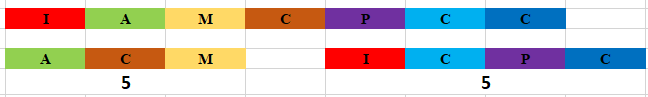
\includegraphics[width=15cm]{images/Screenshot_4.png}
\end{figure}

\end{problem}